\chapter{CPU Scheduling}

\begin{wrapfigure}{r}{0.3\textwidth}
    \centering
    \vspace{-10pt}
    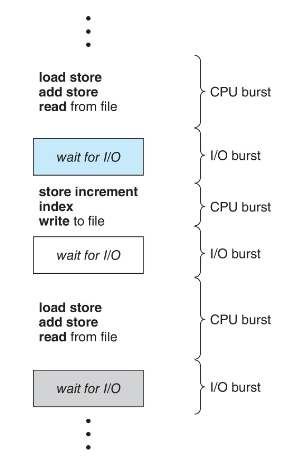
\includegraphics[width=\linewidth]{images/cpu_burst.png}
    \caption{CPU burst and I/O burst}
    \label{fig:cpu_burst_and_io_burst}
    \vspace{-10pt}
\end{wrapfigure}

When we execute one process, typically the CPU is not used all the time, because the process may need to wait for I/O operations to complete. The periods of time when the CPU or the I/O are used are commonly called \textbf{CPU burst} and \textbf{I/O burst}. In a normal computer, there are usually a large number of short CPU bursts and a small number of long CPU bursts.


The CPU scheduler selects from among the process in ready queue, and allocates the CPU to one of them. The selection process is called \textbf{CPU scheduling}. CPU scheduling decision may take place when a process:
\begin{compactitemize}
    \item Switches from running to waiting state
    \item Switches from running to ready state
    \item Switches from waiting to ready
    \item Terminates
\end{compactitemize}
\vspace{0,5cm}
When scheduling takes place only under circumstances 1 and 4, the scheduling is said to be \textbf{non-preemptive}. Otherwise, the scheduling is said to be \textbf{preemptive}.
Under Nonpreemptive scheduling, once the CPU has been allocated to a process, the process keeps the CPU until it releases it either by terminating or by switching to the waiting state.

Preemptive scheduling can lead to race conditions when data are shared among multiple processes. For example, consider two processes that share the same data. While one process is in the middle of updating the data, it may be preempted to allow the second process to execute. If the second process then attempts to read the shared data, it may encounter them in an inconsistent state. This issue will be examined in more detail later.

\begin{wrapfigure}{r}{0.3\textwidth}
    \centering
    \vspace{-10pt}
    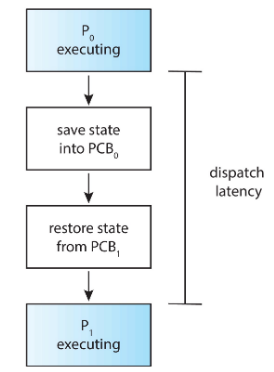
\includegraphics[width=\linewidth]{images/dispacht.png}
    \caption{Dispatcher}
    \label{fig:dispatcher}
    \vspace{-10pt}
\end{wrapfigure}


\textbf{Dispatcher} is the module that gives control of the CPU to the process selected by the short-term scheduler. This involves:
\begin{compactitemize}
    \item Switching context
    \item Switching to user mode
    \item Jumping to the proper location in the user program to restart that program
\end{compactitemize}
The time it takes for the dispatcher to stop one process and start another running is known as the \textbf{dispatch latency}. In some systems, the dispatch latency is considered part of the context switch time.



\textbf{Note:} If we make very frequent context switches, we may spend more time in the dispatcher than in the actual processes. This is called \textbf{thrashing}.

\section{Scheduling Criteria}
When we evaluate a CPU scheduling algorithm, we need to consider the following criteria:
\begin{compactitemize}
    \item \textbf{CPU utilization:} We want to keep the CPU as busy as possible. We want to maximize this value.
    \item \textbf{Throughput:} The number of processes that complete their execution per time unit. We want to maximize this value.
    \item \textbf{Turnaround time:} The total time taken between submission of a process and its completion. We want to minimize this value.
    \item \textbf{Waiting time:} The total time a process has been in the ready queue. We want to minimize this value.
    \item \textbf{Response time:} The time from submission of a request until the first response is produced. We want to minimize this value.
\end{compactitemize}

\subsection{Firsrt-Come, First-Served (FCFS) Scheduling}
In this algorithm, the process that requests the CPU first is allocated the CPU first. The implementation of this algorithm is easily done with a FIFO queue. When a process enters the ready queue, its PCB is linked onto the tail of the queue. When the CPU is free, it is allocated to the process at the head of the queue. This algorithm is non-preemptive.

\begin{table}[H]
    \centering
    \begin{tabular}{|c|c|c|c|}
        \hline
        \textbf{Process} & \textbf{Burst Time} & \textbf{Arrival Time} & \textbf{Waiting Time} \\ 
        \hline
        P1 & 24 & 1 & 0 \\ 
        P2 & 3  & 2 & 24 \\ 
        P3 & 3  & 3 & 27 \\ 
        \hline
    \end{tabular}
    \caption{Process scheduling example}
    \label{tab:process_scheduling}
\end{table}

In the example in Table \ref{tab:process_scheduling}, we have three processes with different burst times and arrival times. The waiting time for each process is calculated as follows:
\begin{compactitemize}
    \item P1: 0 (it starts executing immediately)
    \item P2: 24 (it has to wait for P1 to finish)
    \item P3: 27 (it has to wait for both P1 and P2 to finish)
    \item Average waiting time = (0 + 24 + 27) / 3 = 17
\end{compactitemize}

The Gantt chart in Figure \ref{fig:fcfs_scheduling} illustrates the scheduling of these processes over time.
\begin{figure}[H]
    \centering
    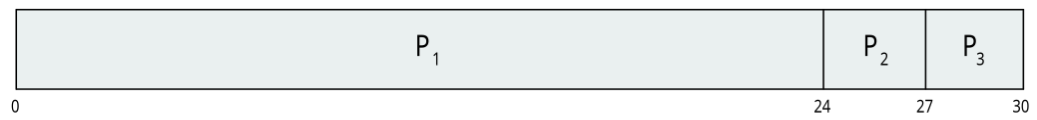
\includegraphics[width=0.6\linewidth]{images/fcfs.png}
    \caption{Example of FCFS scheduling}
    \label{fig:fcfs_scheduling}
\end{figure}

Now, suppose that the process arrivate in the order P2, P3, P1. The waiting times would be:
\begin{compactitemize}
    \item P2: 0 (it starts executing immediately)
    \item P3: 3 (it has to wait for P2 to finish)
    \item P1: 6 (it has to wait for both P2 and P3 to finish)
    \item Average waiting time = (0 + 3 + 6) / 3 = 3
\end{compactitemize}
The Gantt chart in Figure \ref{fig:fcfs_scheduling_2} illustrates the scheduling of these processes over time.
\begin{figure}[H]
    \centering
    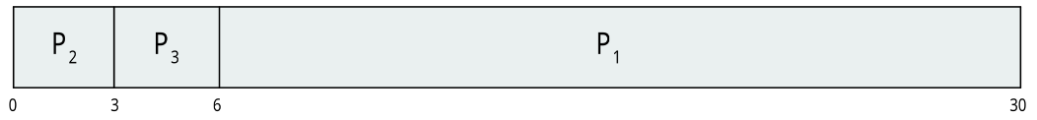
\includegraphics[width=0.6\linewidth]{images/fcfs_order.png}
    \caption{Example of FCFS scheduling with different arrival order}
    \label{fig:fcfs_scheduling_2}
\end{figure}

In this case, the performance are much better. The previous example showed a classic example of the \textbf{convoy effect}, where a long process holds up several short processes. The average waiting time with FCFS can be quite long, depending on the order of process arrival.

\subsection{Shortest-Job-First (SJF) Scheduling}
In this algorithm, the process with the smallest next CPU burst is selected for execution. SJF is optimal, gives minimum average waiting time for a given set of processes. The principal difficulty is how determinate the length of the next CPU burst.
\begin{table}[H]
    \centering
    \begin{tabular}{|c|c|c|}
        \hline
        \textbf{Process} & \textbf{Burst Time} & \textbf{Waiting Time} \\ 
        \hline
        P1 & 6 & 3 \\ 
        P2 & 8 & 16 \\ 
        P3 & 7 & 9 \\ 
        P4 & 3 & 0 \\ 
        \hline
    \end{tabular}
    \caption{Shortest-job-First scheduling example}
    \label{tab:process_scheduling_2}
\end{table}
In the example in Table \ref{tab:process_scheduling_2}, we have four processes with different burst times. The waiting time for each process is calculated as follows:
\begin{compactitemize}
    \item P1: 3 (it has to wait for P4 to finish)
    \item P2: 16 (it has to wait for P4, P1 and P3 to finish)
    \item P3: 9 (it has to wait for P4 and P1 to finish)
    \item P4: 0 (it starts executing immediately)
    \item Average waiting time = (3 + 16 + 9 + 0) / 4 = 7
\end{compactitemize}
The Gantt chart in Figure \ref{fig:sjf_scheduling} illustrates the scheduling of these processes over time.
\begin{figure}[H]
    \centering
    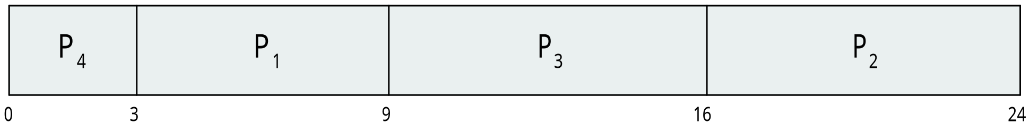
\includegraphics[width=0.6\linewidth]{images/sjf_scheduling.png}
    \caption{Example of Shortest-Job-First scheduling}
    \label{fig:sjf_scheduling}
\end{figure}

Now let's a look how can we predict the length of the next CPU burst. One method is to use the length of previous CPU bursts. We can use exponential averaging to predict the length of the next CPU burst:
\[
    \tau_{n+1} = \alpha t_n + (1 - \alpha) \tau_n
\]
where:
\begin{compactitemize}
    \item $\tau_{n+1}$ is the predicted length of the next CPU burst
    \item $t_n$ is the actual length of the previous CPU burst
    \item $\tau_n$ is the predicted length of the previous CPU burst
    \item $\alpha$ is a constant between 0 and 1
\end{compactitemize}
The value of $\alpha$ determines the weight given to the most recent CPU burst. A higher value of $\alpha$ gives more weight to the most recent burst, while a lower value gives more weight to the past bursts. Commonly used values for $\alpha$ is 0.5.
If $alpha$ is 0, then the prediction is based entirely on the past history. If $\alpha$ is 1, then the prediction is based entirely on the most recent burst.
if we expand the equation, we get:
\[
\tau_{n+1} = \alpha t_n + (1 - \alpha)\alpha t_{n-1} + \dots 
+ (1 - \alpha)^j \alpha t_{n-j} + \dots 
+ (1 - \alpha)^{n+1} \tau_0
\]

where $\tau_0$ is the initial guess for the length of the CPU burst.Since both $\alpha$ and $(1 - \alpha)$ are less than or equal to $1$, each successive term in the equation contributes less to the final value than the one before it. In other words, as we move further back in time (to older $t_{n-1}, t_{n-2}, \dots$), each term is multiplied by an additional factor of $(1 - \alpha)$, which reduces its weight.

This means that \textbf{recent observations} (such as $t_n$) have a stronger influence on the predicted value $\tau_{n+1}$, while \textbf{older observations} gradually become less significant because their weights decrease exponentially.

\textbf{Note:} The burst prediction formula is unique to each process. Each process has its own $\tau$ value that is updated after each CPU burst. If the process has never been executed before, we can set $\tau_0$ to an arbitrary value, such as the average CPU burst time for all processes.
\begin{figure}[H]
    \centering
    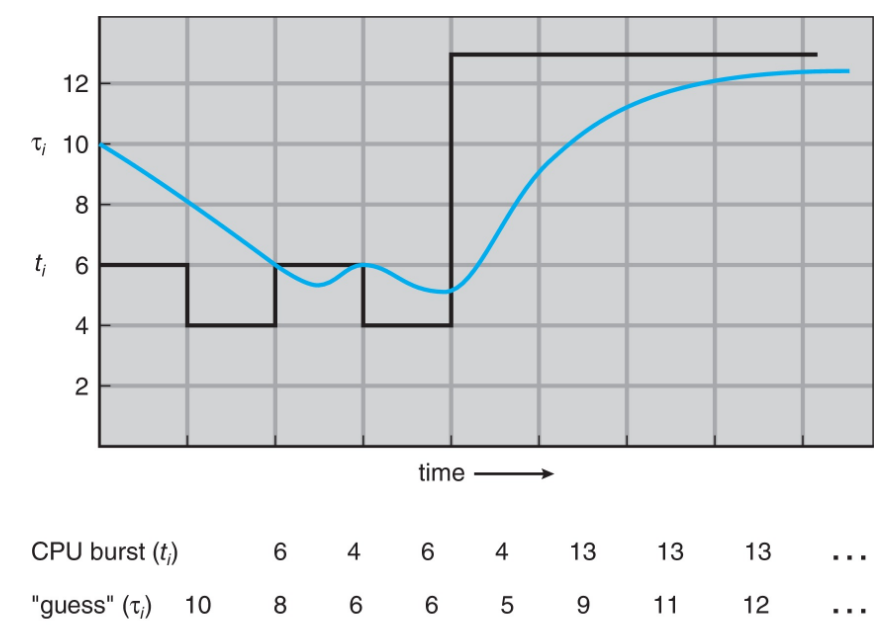
\includegraphics[width=0.6\linewidth]{images/cpu_pred.png}
    \caption{Example of CPU burst prediction}
    \label{fig:cpu_burst_prediction}
\end{figure}

\subsection{Shortest-Remaining-Time-First (SRTF)}
Is the preemptive varsion of SJF. When a new process arrives in the ready queue, the decision on which process to schedule next id redon using the SJF criteria. If the new process has a CPU burst length less than the remaining time of the currently executing process, the current process is preempted and the new process is scheduled.
\begin{table}[H]
    \centering
    \begin{tabular}{|c|c|c|c|}
        \hline
        \textbf{Process} & \textbf{Arrival Time} & \textbf{Burst Time} & \textbf{Waiting Time} \\ 
        \hline
        P1 & 0 & 8 & 10--1 \\ 
        P2 & 1 & 4 & 1--1 \\ 
        P3 & 2 & 9 & 17--2 \\ 
        P4 & 3 & 5 & 5--3 \\ 
        \hline
    \end{tabular}
    \caption{Process scheduling example}
    \label{tab:process_scheduling_example}
\end{table}

In the example in Table \ref{tab:process_scheduling_example}, we have four processes with different burst times and arrival times. The waiting time for each process is calculated as follows:
\begin{compactitemize}
    \item P1: 10 - 1 = 9 (it has to wait for P2 and P4 to finish)
    \item P2: 1 - 1 = 0 (it starts executing immediately after arriving)
    \item P3: 17 - 2 = 15 (it has to wait for P1, P2 and P4 to finish)
    \item P4: 5 - 3 = 2 (it has to wait for P2 to finish)
    \item Average waiting time = (9 + 0 + 15 + 2) / 4 = 6.5
\end{compactitemize}
The Gantt chart in Figure \ref{fig:srtf_scheduling} illustrates the scheduling of these processes over time.
\begin{figure}[H]
    \centering
    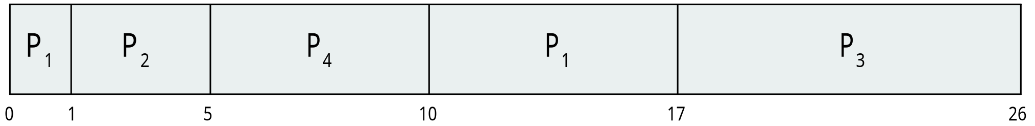
\includegraphics[width=0.6\linewidth]{images/srtf_scheduling.png}
    \caption{Example of Shortest-Remaining-Time-First scheduling}
    \label{fig:srtf_scheduling}
\end{figure}

\subsection{Round Robin (RR) Scheduling}
Each process gets a small unit of CPU time, called the time quantum $q$, which usually ranges between 10 and 100 milliseconds. After this time has elapsed, the process is preempted and added to the end of the ready queue. 

Assuming there are $n$ processes in the ready queue and the time quantum is $q$, each process receives $\frac{1}{n}$ of the CPU time in chunks of at most $q$ time units at once. Consequently, no process waits more than $(n - 1)q$ time units before getting the CPU again. A timer interrupts the system after each quantum to schedule the next process.

Regarding performance, if $q$ is large, the scheduling algorithm behaves like FIFO (First-Come, First-Served), whereas if $q$ is small, it approaches Round Robin (RR) scheduling. It is important to note that $q$ must be sufficiently large compared to the context switch time; otherwise, the overhead introduced by frequent context switches becomes too high.
\begin{table}[H]
    \centering
    \begin{tabular}{|c|c|}
        \hline
        \textbf{Process} & \textbf{Burst Time} \\ 
        \hline
        P1 & 24 \\ 
        P2 & 3 \\ 
        P3 & 3 \\ 
        \hline
    \end{tabular}
    \caption{Example of RR with q=4}
    \label{tab:process_burst_times}
\end{table}
The Gantt chart in Figure \ref{fig:rr_scheduling} illustrates the scheduling of these processes over time with a time quantum of 4.
\begin{figure}[H]
    \centering
    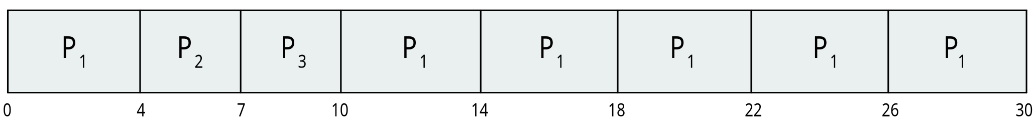
\includegraphics[width=0.6\linewidth]{images/rr_scheduling.png}
    \caption{Example of Round-Robin scheduling}
    \label{fig:rr_scheduling}
\end{figure}
Typically, the Round Robin scheduling algorithm results in a higher average turnaround time compared to the Shortest Job First (SJF) algorithm, but it provides better response time. The time quantum $q$ should be large compared to the context switch time. In general, $q$ is measured in milliseconds, while the context switch time is measured in microseconds.
\begin{figure}[H]
    \centering
    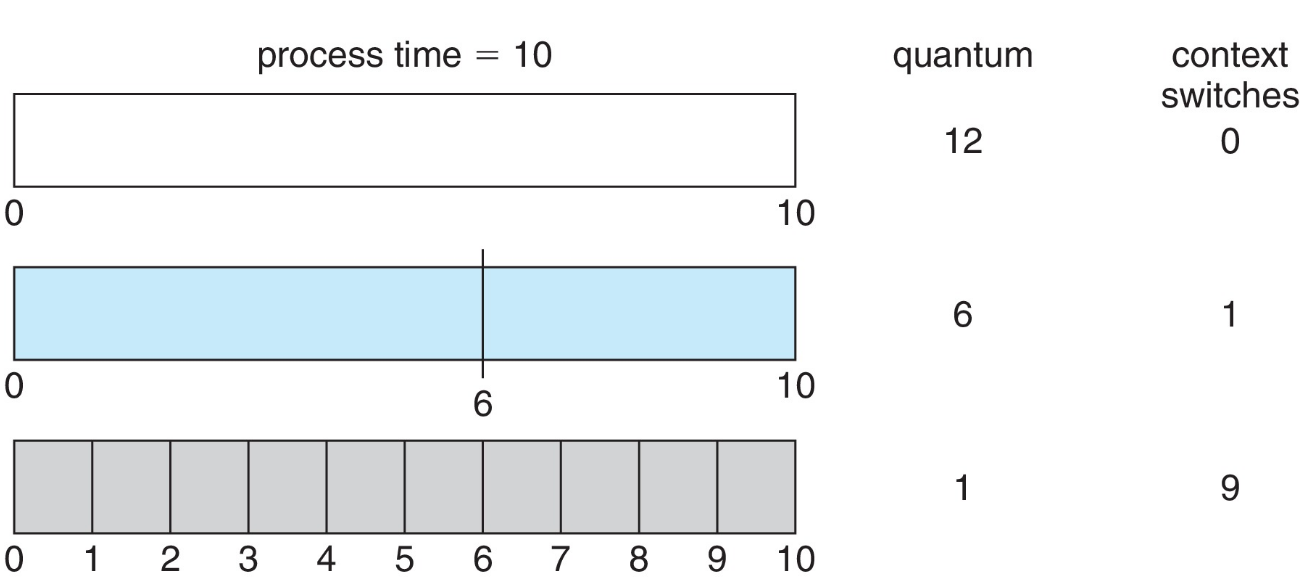
\includegraphics[width=0.6\linewidth]{images/quantum.png}
    \caption{Different time quantums}
    \label{fig:different_time_quantums}
\end{figure}

\begin{wrapfigure}{r}{0.2\textwidth}
    \centering
    \vspace{-10pt}
    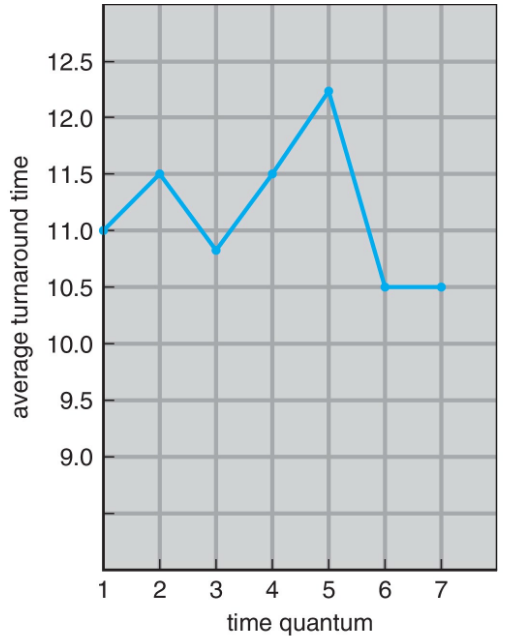
\includegraphics[width=\linewidth]{images/turnaround_time.png}
    \caption{Turnaround Time vs. q}
    \label{fig:turnaround_time_vs_q}
    \vspace{-10pt}
\end{wrapfigure}
The turnaround time depends on the time quantum $q$, although this dependency is not necessarily linear. As a general rule of thumb, approximately 80\% of CPU bursts should be shorter than the value of $q$.

\subsection{Priority Scheduling}
A priority number (an integer) is associated with each process. The CPU is allocated to the process with the highest priority, where a smaller integer value represents a higher priority. Priority scheduling can be either preemptive or nonpreemptive. 

The Shortest Job First (SJF) algorithm is a special case of priority scheduling in which the priority is the inverse of the predicted next CPU burst time. However, this approach can lead to the problem of \textbf{starvation}, where low-priority processes may never get executed. A common solution to this issue is \textbf{aging}, a technique in which the priority of a process gradually increases as time progresses, ensuring that every process eventually gets CPU time.
\begin{table}[H]
    \centering
    \begin{tabular}{|c|c|c|}
        \hline
        \textbf{Process} & \textbf{Burst Time} & \textbf{Priority} \\ 
        \hline
        P1 & 10 & 3 \\ 
        P2 & 1  & 1 \\ 
        P3 & 2  & 4 \\ 
        P4 & 1  & 5 \\ 
        P5 & 5  & 2 \\ 
        \hline
    \end{tabular}
    \caption{Processes with burst times and priorities}
    \label{tab:process_priority}
\end{table}
In the example in Table \ref{tab:process_priority}, we have five processes with different burst times and priorities. The Gantt chart in Figure \ref{fig:priority_scheduling} illustrates the scheduling of these processes over time using non-preemptive priority scheduling. The average waiting time is equal to 8.2 .
\begin{figure}[H]
    \centering
    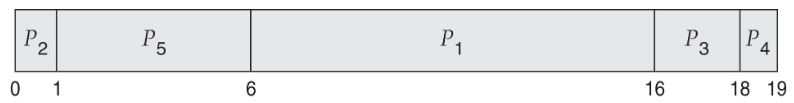
\includegraphics[width=0.6\linewidth]{images/priority_scheduling.png}
    \caption{Example of Priority scheduling}
    \label{fig:priority_scheduling}
\end{figure}

If more than one process has the same priority, we can use  Round Robin, as in the example in table \ref{tab:process_priority_2}, where P1 and P5 have the same priority.
\begin{table}[H]
    \centering
    \begin{tabular}{|c|c|c|}
        \hline
        \textbf{Process} & \textbf{Burst Time} & \textbf{Priority} \\ 
        \hline
        P1 & 4 & 3 \\ 
        P2 & 5 & 2 \\ 
        P3 & 8 & 2 \\ 
        P4 & 7 & 1 \\ 
        P5 & 3 & 3 \\ 
        \hline
    \end{tabular}
    \caption{Processes with burst times and priorities, but P1 and P5 have the same priority}
    \label{tab:process_priority_2}
\end{table}
The Gantt chart in Figure \ref{fig:priority_scheduling_2} illustrates the scheduling of these processes over time using RR for processes with the same priority. The q used is equal to 2.
\begin{figure}[H]
    \centering
    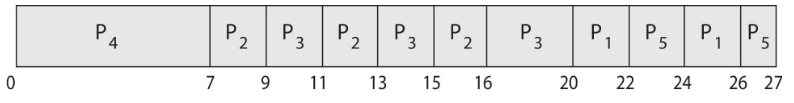
\includegraphics[width=0.6\linewidth]{images/priority_scheduling_2.png}
    \caption{Example of Priority scheduling with RR for processes with the same priority}
    \label{fig:priority_scheduling_2}
\end{figure}

\section{Scheduling with Multiple queues}